\documentclass{amsart}
\usepackage[ruled,vlined]{algorithm2e}
\usepackage{amsmath}
\usepackage[margin=1in]{geometry}
\DeclareMathOperator*{\argmax}{arg\,max}
\DeclareMathOperator*{\argmin}{arg\,min}
\usepackage{adjustbox}
\usepackage{ifpdf}
\usepackage{url}
\usepackage{graphicx}
\usepackage{float}
\usepackage{caption}
\usepackage{subcaption}
\usepackage{amsfonts}
\title{Project 6 \\ Reinforcement Learning}
\author{David Atlas}


\begin{document}
    \begin{abstract}
    This paper will introduce basic concepts in reinforcement
    learning, including three algorithms for finding policies: Value Iteration, Q-Learning and SARSA.
        The paper will introduce a simulated race-track environment, and present results on
        learning a policy in the environment. It would be expected that the algorithms will
        have an easier time learning smaller environments and simpler crash outcome
        variants, and that the Q-Learning/SARSA
        approach will have more success in the larger environments, as they do not
        require exhaustive updates to the space, and are more easily able to hone a good policy
        without visiting every space on the track.
    The experiments validate this hypothesis, as the algorithms are able to find good policies
        on the smaller tracks, and are more successful with the simpler crash variant.
    \end{abstract}
    \maketitle

    \section{Problem Statement \& Hypothesis}
    This paper introduces several core concepts in reinforcement learning. Reinforcement
    learning attempts to solve the problem of determining an optimal policy for an agent at any
    given state in an environment, given some reward structure.

    The basic problem in reinforcement learning is a Markov Decision Process (MDP).
    In an MDP, the optimal decision depends only on the current state of the agent. At each time step,
    after an action is taken, a reward is given.

    Specifically, in this paper, the agent will be a racecar on a racetrack with several different
    elements:
    \begin{itemize}
        \item A set of starting locations for the car.
        \item A set of finish line locations for the car.
        \item A set of out-of-bounds markers for the car.
    \end{itemize}

    The problem of solving the policy involves determining the optimal acceleration at each location of the racetrack.

    Additionally, there is an element of randomness involved - at each step, after an acceleration
    action is chosen, there is only an 80\% chance of it happening as expected.

    There are 3 tracks included in the problem, each with increasing size and difficulty:
    \begin{enumerate}
        \item L-Track
        \item O-Track
        \item R-Track
    \end{enumerate}

    The hypothesis is that all of the algorithms should be able to solve all of the tracks, as they all meet the
    Markov criteria (all information needed is encoded in the current state). However, the algorithms take quite a
    while to train, and so there may be difficulties finding an optimal policy for all of the tracks.

    Note that each track has two variants - in the first variant, which will be called the harsh variant,
    if the car hits the out-of-bounds marker, it is returned to the starting location. In the second variant,
    which will be called the simpler variant, the car is simply returned to its last location with velocity of 0.
    It would be expected that the harsh variant is more difficult to train, as restarting from the beginning of
    the track would give potentially large policy values to states that are close to the finish line. As the randomness
    of the track could cause a crash on what would have otherwise been a good decision, it will take more iterations  to
    converge to the correct values.

    \section{Description of Algorithms}
    \subsection{Notation}
    The following concepts will be useful in describing the algorithms below:
    \begin{itemize}
        \item $S$ is the set of states in the environment.
        \item $A$ is the set of actions that can be executed by the agent.
        \item Policy $\pi(s)$ is a mapping from state $s$ to action $a$. This can be thought of as the
        guidebook for the agent, telling it what to do at each state in the environment.
        \item $Q(s, a)$ is a mapping that dictates the expected reward for choosing action $a$ from state $s$.
        \item $\gamma$ is the discount rate, or the amount by which a future reward is discounted. A reward
        in $t$ iterations gets discounted by a factor of $\gamma^t$.
    \end{itemize}

    \subsection{Bellman's Equation}
    The solution to an MDP can be written as
    \begin{align}
        V^*(s_t)
        &= \argmax_{a_t} Q^*(s_t, a_t) \\
        &= \argmax_{a_t} E[r_{t+1} \sum_{t=1}^\infty \gamma^{i-1} r_t + i + 1] \\
        &= E[r_{t+1}] + \gamma \sum_{s_{t+1}} P(s_{t+1} \mid s_t, a_t) \argmax_{a_{t+1}} Q^*(s_{t+1}, a_{t+1}).
        \label{bellman}
    \end{align}
    Equation~\ref{bellman} is known as Bellman's Equation. The terms can be thought of intuitively as
    the "correct" value for a given state-action pair $Q(s_t, a_t)$ at time $t$ as the reward of executing
    the action ($r_{t+1}$), as well as the sum of all expected future rewards from states $s_{t+1}$,
    weighted by the likelihood of ending up in the state after executing action $a_t$ from $s_t$. This
    accounts for any randomness in the environment that leads to probablistic transition dynamics after
    executing $a_t$ from $s_t$.


    \subsection{Value Iteration}
    The Value Iteration algorithm\cite{value_iteration} attempts to find
    $Q^*(s, a)$ by iteratively updating each entry in $Q$ as the sum of the current value and the discounted value
    from executing each action. The algorithm appears as follows:

    \begin{algorithm}[H]
    \SetAlgoLined
        \KwResult{$Q^*(s, a)$}
         Initialize $Q(s, a)$ to arbitrary values\;
        \For{$i\gets0$ \KwTo Number of Iterations}{
            \For{$s \in S$}{
                \For{$a \in A$}{
                    $Q(s, a) \gets E\left[r \mid s, a\right] + \gamma \sum_{s^\prime \in S} P(s^\prime \mid s, a) V(s^\prime)$ \;
                }
            }
        }
     \caption{Value Iteration}
    \label{value_iteration_algorithm}
    \end{algorithm}


    The intuition here is that at each iteration, each state-action pair updates the estimate of its value by looking
    at the states it would end up, and their respective values. It then discounts backwards and add the reward of the
    future state to its value. After many iterations through all the state-action pairs, the algorithm converges
    to values close to the optimal $Q^*(s, a)$.

    \subsection{Q-Learning}
    The next algorithm implemented was the Q-Learning algorithm\cite{q_learning}, which (as might be expected) is another algorithm for
    learning $Q^*(s, a)$. Before introducing the algorithm, the $\epsilon$-greedy action selection policy must be
    introduced. For a state $s_t$, the $\epsilon$-greedy policy selects the optimal (as of time $t$) action with
    probability $1-\epsilon$, while selecting a random action with probablity $\epsilon$. This can be thought of as
    a tuning parameter, where the agent will spend more time experimenting when $\epsilon$ is higher. This is
    useful in iterative training because it would be undesirable for the agent to choose the optimal policy
    at the outset, as it will be randomly initialized.

    With that, the Q-Learning algorithm is shown in Algorithm~\ref{q_learning_algo_block}.


    \begin{algorithm}[H]
    \SetAlgoLined
        \KwResult{$Q^*(s, a)$}
        Initialize $Q(s, a)$ to arbitrary values\;
        \For{$i\gets0$ \KwTo Number of Episodes}{
            $s \gets s_0$ (a starting state)\;
            \While{$s$ is not a terminal state}{
                Choose $a$ via $\epsilon$-greedy selection\;
                Get $r$ and $s^\prime$ from applying $a$ in $s$\;
                $Q(s, a) \gets Q(s, a) + \eta (r + \gamma \argmax_{a^\prime} Q(s^\prime, a^\prime) - Q(s, a))$\;
                $s \gets s^\prime$
            }
        }
     \caption{Q-Learning}
    \label{q_learning_algo_block}
    \end{algorithm}

    The intuition behind algorithm \ref{q_learning_algo} is to use the $\epsilon$-greedy action selection to explore the space, while
    estimating $Q(s, a)$ as a mix between its current value and the approximate additional reward that would be come
    from taking action $a$, and the proceeding in accordance with the policy at the new state, $s^\prime$.
    The big difference between Q-Learning and Value Iteration is that Q-Learning uses episodes, in which the agent
    makes a sequence of decisions from the beginning to the end, updating the policy along the way, whereas Value Iteration
    updates each state-action pair on each iteration. This means that for very large state spaces, Q-Learning may have
    an easier time learning a good policy, while Value Iteration would require alot of computational resources to
    update each state at each iteration.

    \subsection{SARSA}
    The last algorithm presented here is SARSA (State-Action-Reward-State-Action)\cite{sarsa}. This is known as an
    on-policy learning algorithm, as the policy is used to determine not only the immediate action $a$, but also
    the succeeding one, $a^\prime$. This is in contrast to Q-Learning, in which the policy only determines $a$,
    and the ensuing reward is estimated by the approximation of the optimal choice at state $Q(s^\prime, a)$.
    However, the agent does not necessarily make that optimal choice. Beyond this difference, the
    algorithms are quite similar. SARSA is shown in Algorithm~\ref{sarsa_algo_block}.

    \begin{algorithm}[H]
    \SetAlgoLined
        \KwResult{$Q^*(s, a)$}
         Initialize $Q(s, a)$ to arbitrary values\;
        \For{$i\gets0$ \KwTo Number of Episodes}{
            $s \gets s_0$ (a starting state)\;
            Choose $a$ via $\epsilon$-greedy selection\;
            \While{$s$ is not a terminal state}{
                Get $r$ and $s^\prime$ from applying $a$ in $s$\;
                Choose $a^\prime$ from $\epsilon$-greedy selection in $s^\prime$\;
                $Q(s, a) \gets Q(s, a) + \eta (r + \gamma \argmax_{a^\prime} Q(s^\prime, a^\prime) - Q(s, a))$\;
                $s \gets s^\prime$\;
                $a \gets a^\prime$\;
            }
        }
    \caption{Q-Learning}
    \label{sarsa_algo_block}
    \end{algorithm}

    \subsection{Experimental Approach}
    There were 3 environments used in each experiment:
    \begin{enumerate}
    \item L-Shaped Track
    \item O-Shaped Track
    \item R-Shaped Track
    \end{enumerate}

    For each environment, Value Iteration, Q-Learning and SARSA were all applied to the environment. Each algorithm
    was allowed to train for a variable number of iterations, until performance converged to good solution. To be
    clear, a good solution here implies going from start to finish in a number of steps proportional to the difficulty
    of tracing such a path.

    The algorithms have hyperparameters - all of the algorithms include a discount factor, which is the amount by which
    a future reward is discounted back to the present time step. Both Q-Learning and SARSA include a
    learning rate, which is the proportion of the temporal difference that is added back to the current tally of the
    expected reward in a given state. Additionally, Q-Learning and SARSA have an $\epsilon$ parameter that dictates
    the likelihood of choosing a random action in each state.

    Due to the time-consuming nature of training the algorithms, it would be preferable to avoid exhaustive
    experimentation with respect to the hyperparameters. Therefore, for track-algorithm pairs that
    did not require any tuning to converge to a good solution, values were chosen based on some intuition about the
    relationships between the hyperparameters and the training process. This included all variants of all algorithms
    for the L-track and the O-track, and SARSA and Q-Learning for the R-track under the non-harsh
    crash variant. For the $\epsilon$-greedy policy, the larger of $\frac{1}{T}$ and $.25$ was used to ensure
    sufficient exploration of the space.

    For the remaining combinations, some light experimental tuning was used to find more preferable values. However,
    this approach was not useful, and the algorithms were not converging in a reasonable time. Therefore, a
    "pre-training" approach was used, in which the starting policy was the policy found by SARSA
    under the non-harsh variant.


    \subsection{Algorithm Results}
    The results of the algorithms can be found below in Table~\ref{results_tab}
    \begin{table}
    \begin{adjustbox}{width=1\textwidth}
        \small
    \begin{tabular}{lllcccc}
        Track & Algorithm & Crash Variant & Discount Factor & Learning Rate & Number of Training Iterations & Average Steps to Solve \\
        \hline
        L & Value Iteration & Harsh       & .7              & N/A           & 250 & NA \\
        L & Value Iteration & Non-Harsh   & .8              & N/A           & 100 & NA \\
        L & Q-Learning      & Harsh       & .5              & .2           & 100000 & NA \\
        L & Q-Learning      & Non-Harsh   & .5              & .2           & 40000 & NA \\
        L & SARSA           & Harsh       & .5              & .2           & 125000 & NA \\
        L & SARSA           & Non-Harsh   & .5              & .2           & 4000 & NA \\
        O & Value Iteration & Harsh       & .7              & N/A           & 1000 & NA \\
        O & Value Iteration & Non-Harsh   & .8              & N/A           & 500 & NA \\
        O & Q-Learning      & Harsh       & .5              & .2           & 175000 & NA \\
        O & Q-Learning      & Non-Harsh   & .5              & .2           & 75000 & NA \\
        O & SARSA           & Harsh       & .5              & .2           & 200000 & NA \\
        O & SARSA           & Non-Harsh   & .5              & .2           & 4000 & NA \\


    \end{tabular}
    \end{adjustbox}
    \label{results_tab}
    \end{table}


    \begin{figure}
    \centering
    \begin{subfigure}[t]{0.3\textwidth}
    \centering
    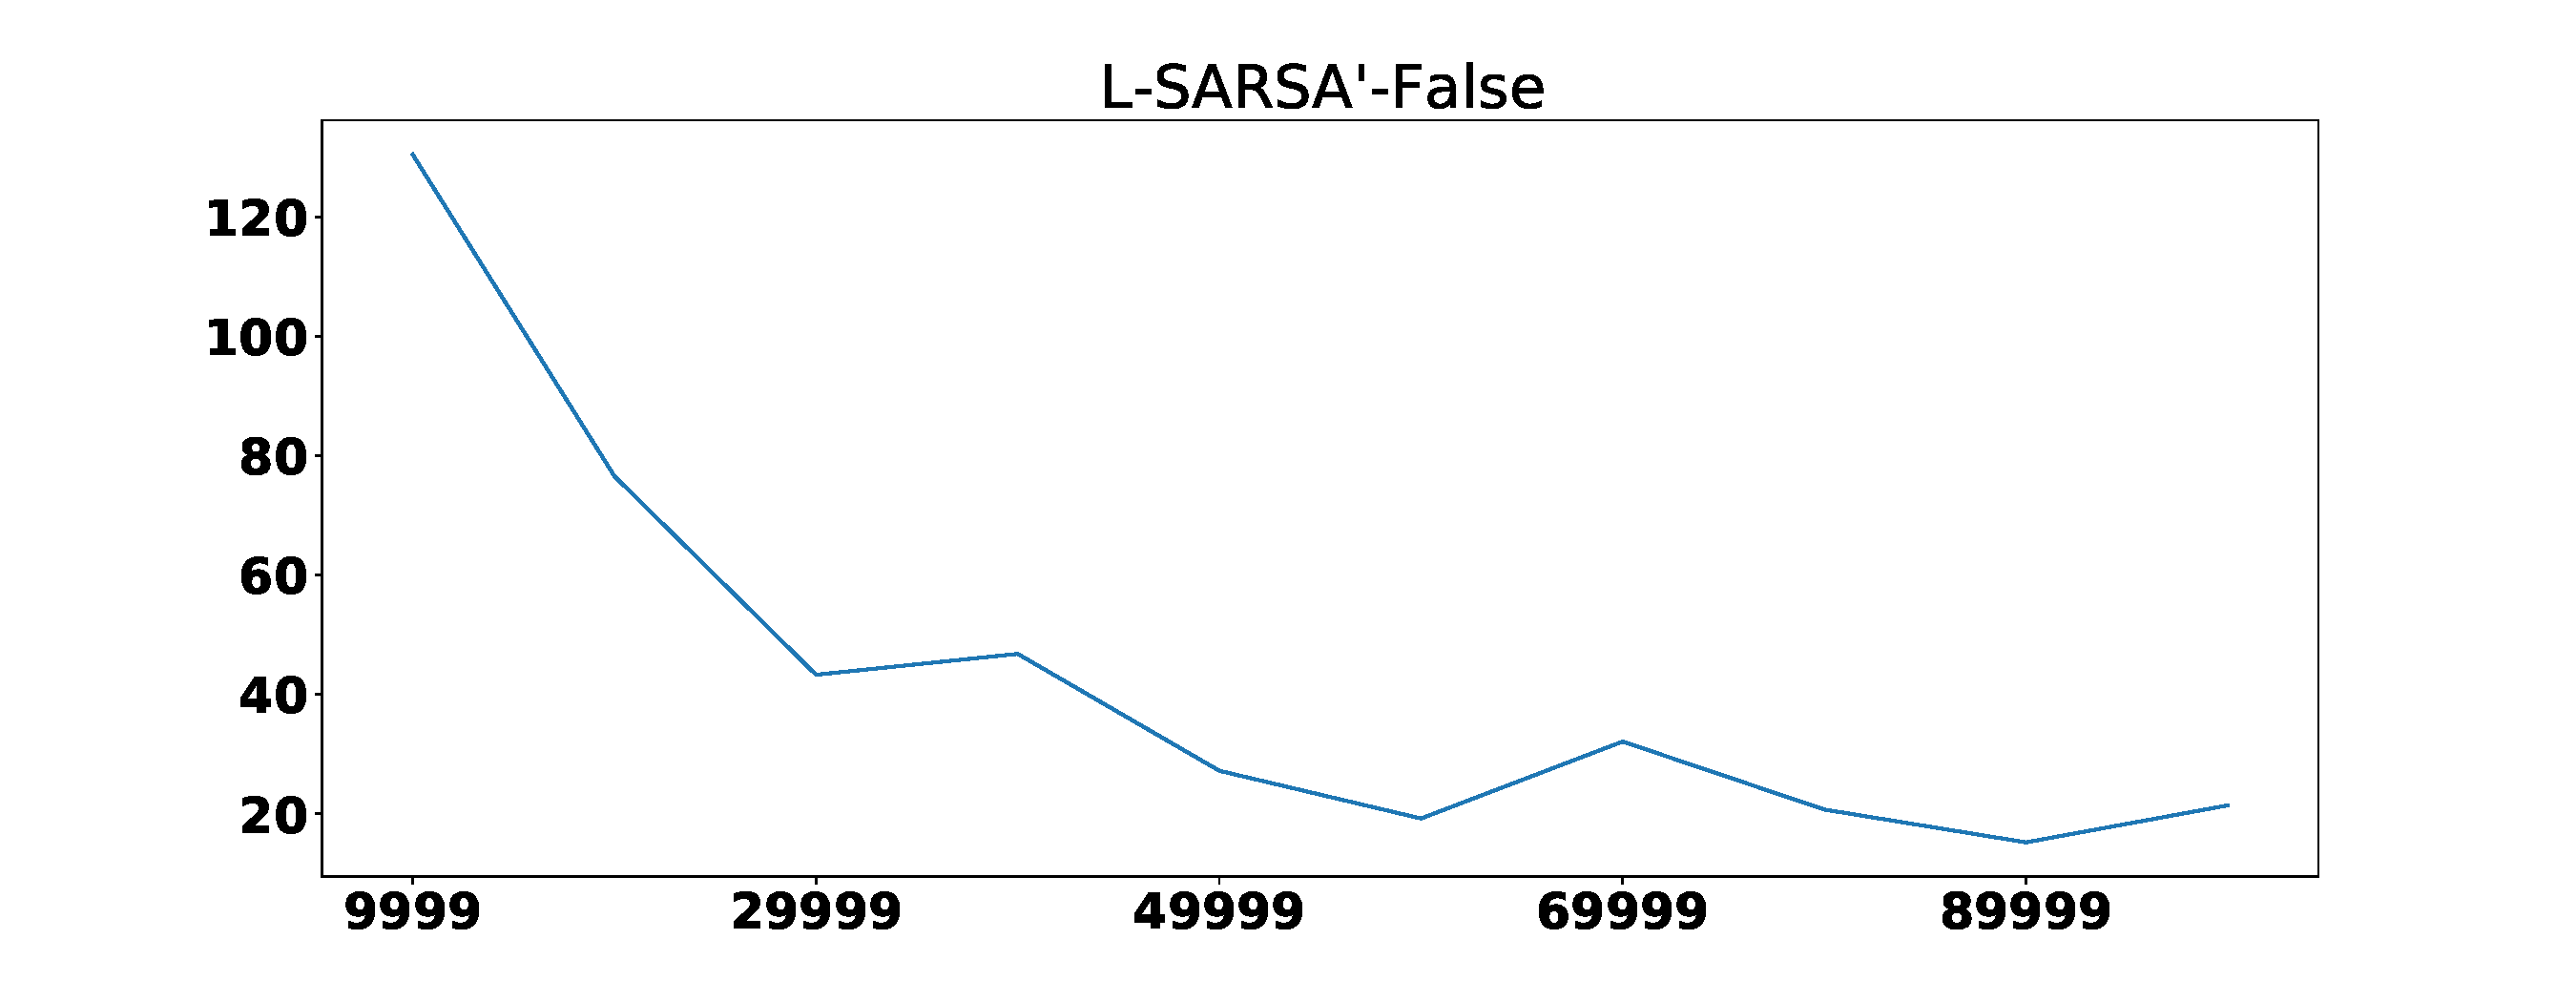
\includegraphics[width=\textwidth]{Ltrack_2_learning_rate.pdf}
    \end{subfigure}
    \begin{subfigure}[t]{0.3\textwidth}
    \centering
    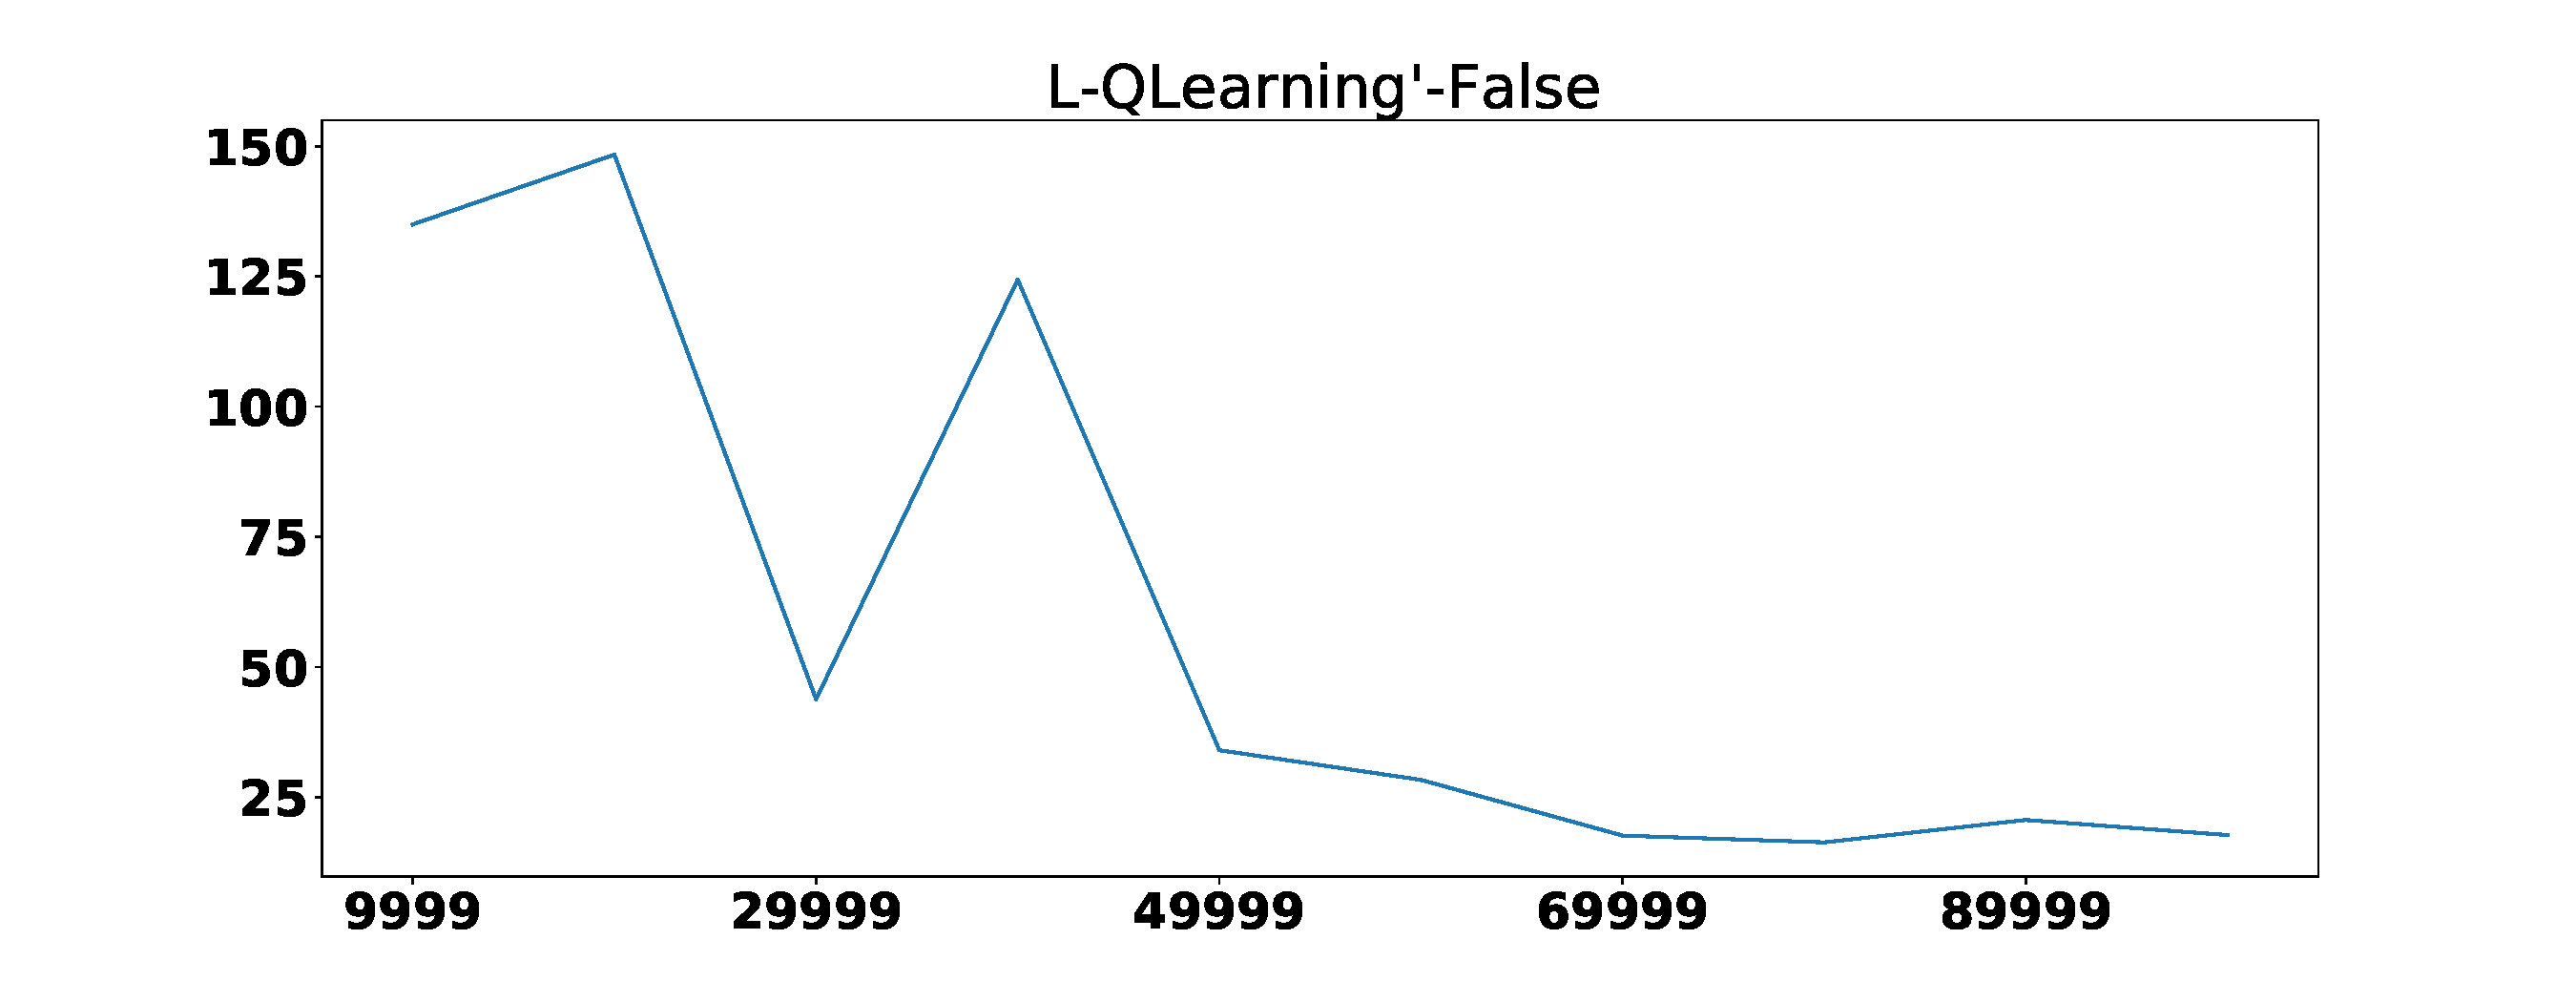
\includegraphics[width=\textwidth]{Ltrack_3_learning_rate.pdf}
    \end{subfigure}
    \begin{subfigure}[t]{0.3\textwidth}
    \centering
    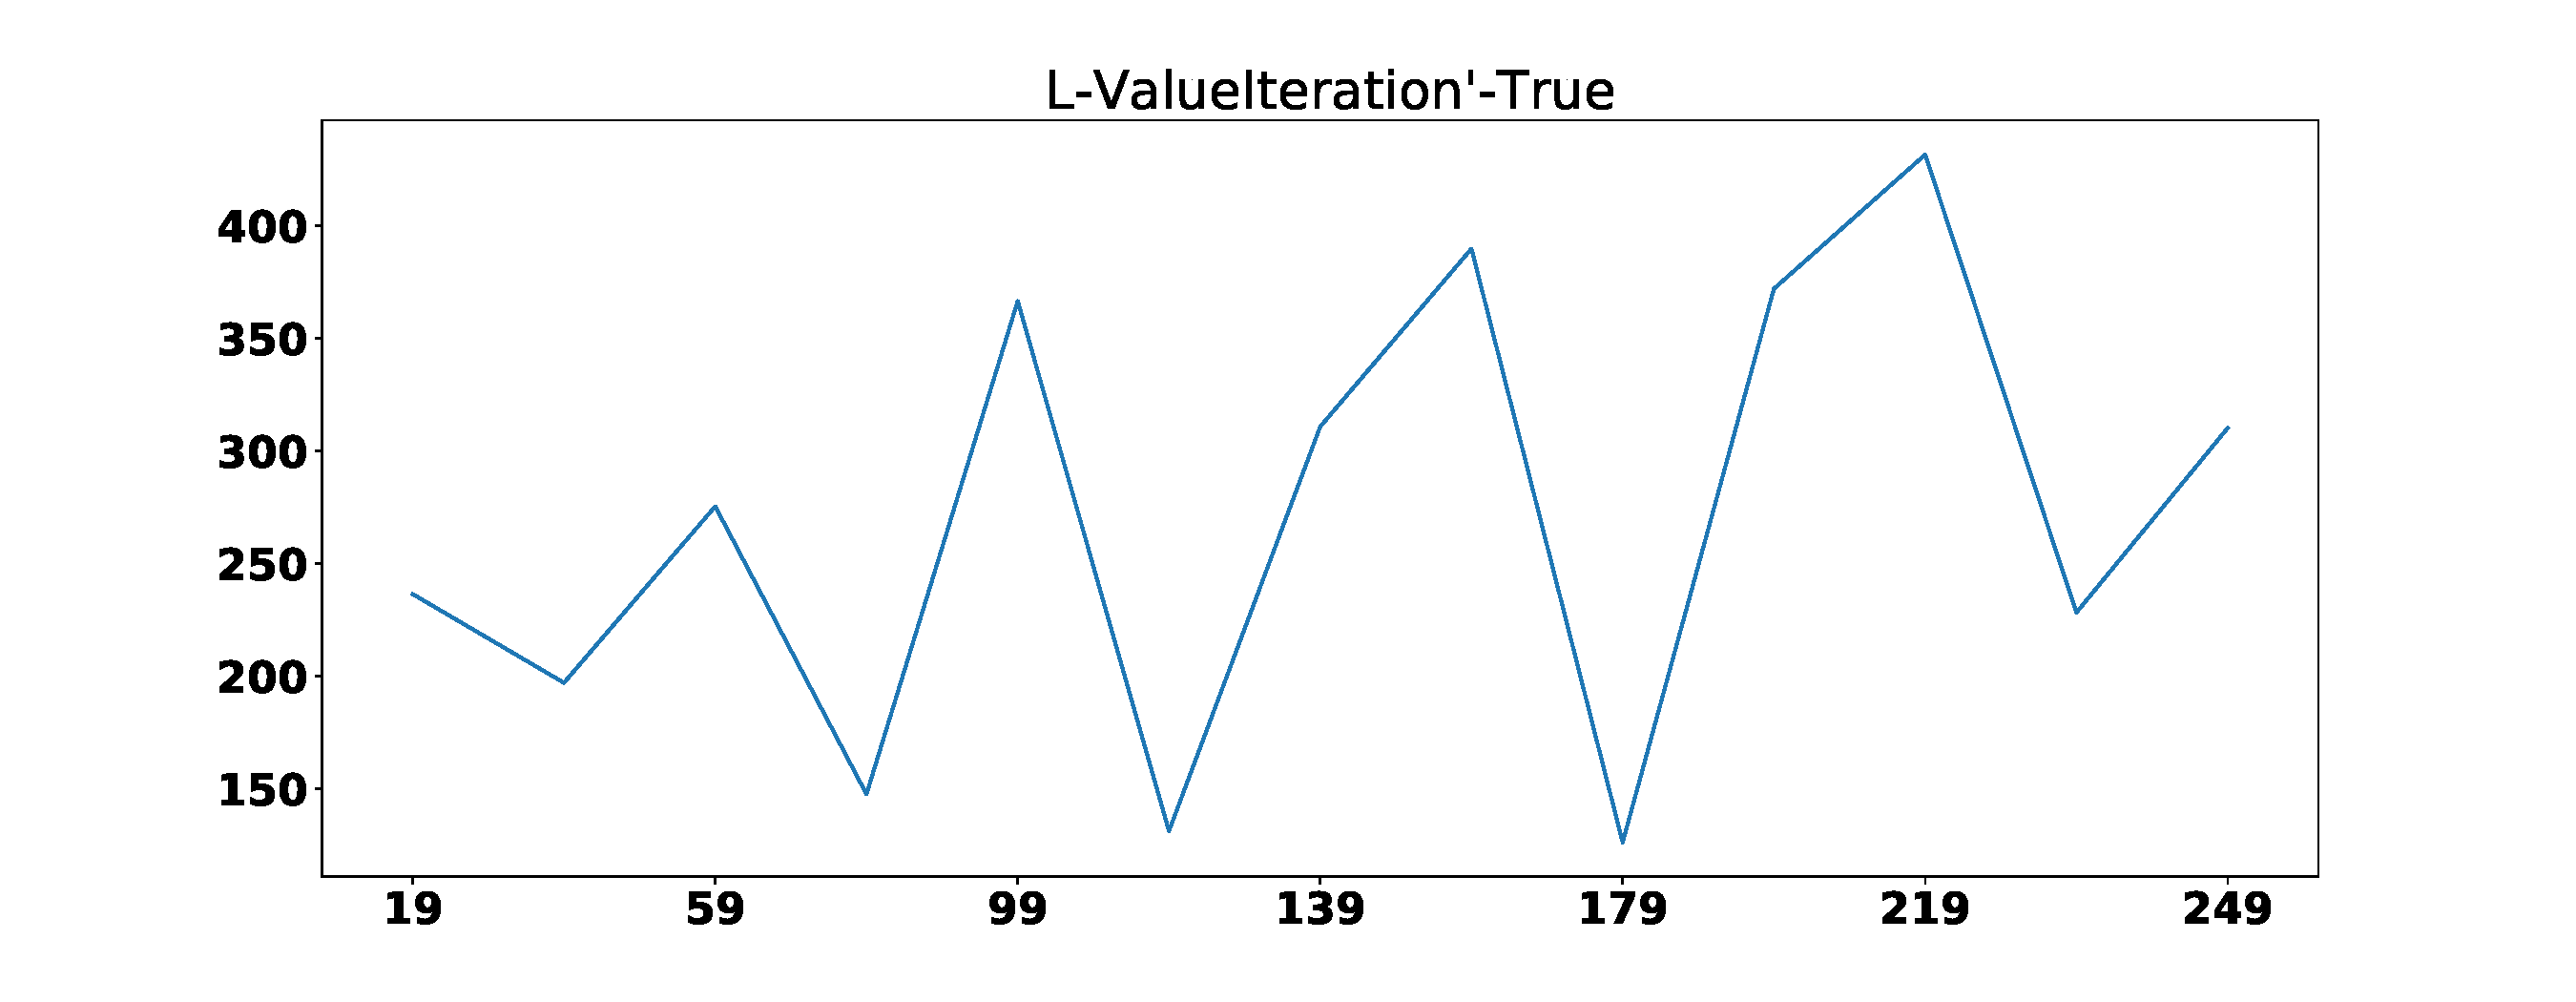
\includegraphics[width=\textwidth]{Ltrack_6_learning_rate.pdf}
    \end{subfigure}
    \begin{subfigure}[t]{0.3\textwidth}
    \centering
    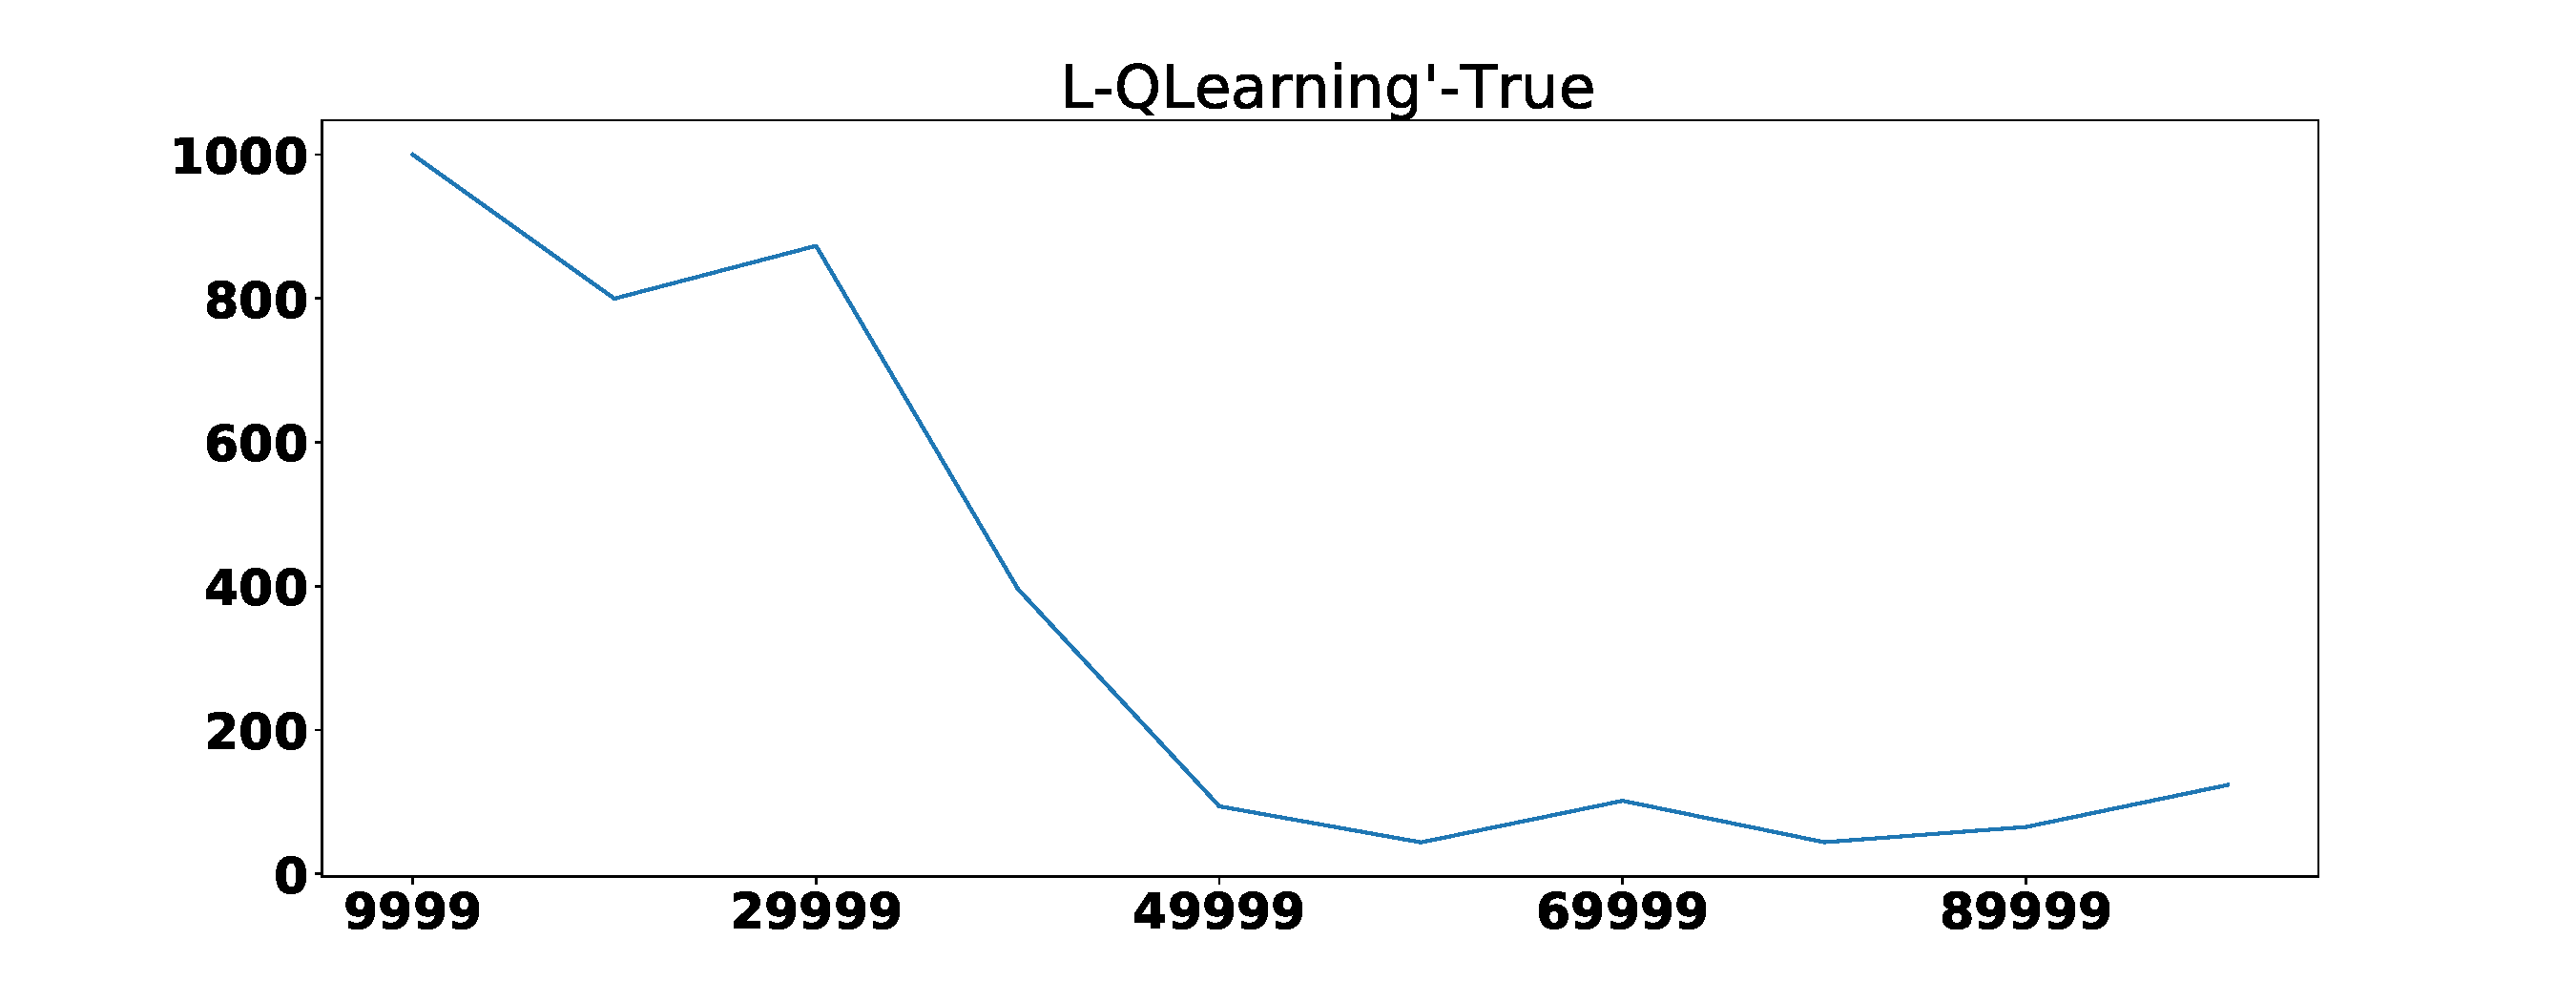
\includegraphics[width=\textwidth]{Ltrack_5_learning_rate.pdf}
    \end{subfigure}
    \begin{subfigure}[t]{0.3\textwidth}
    \centering
    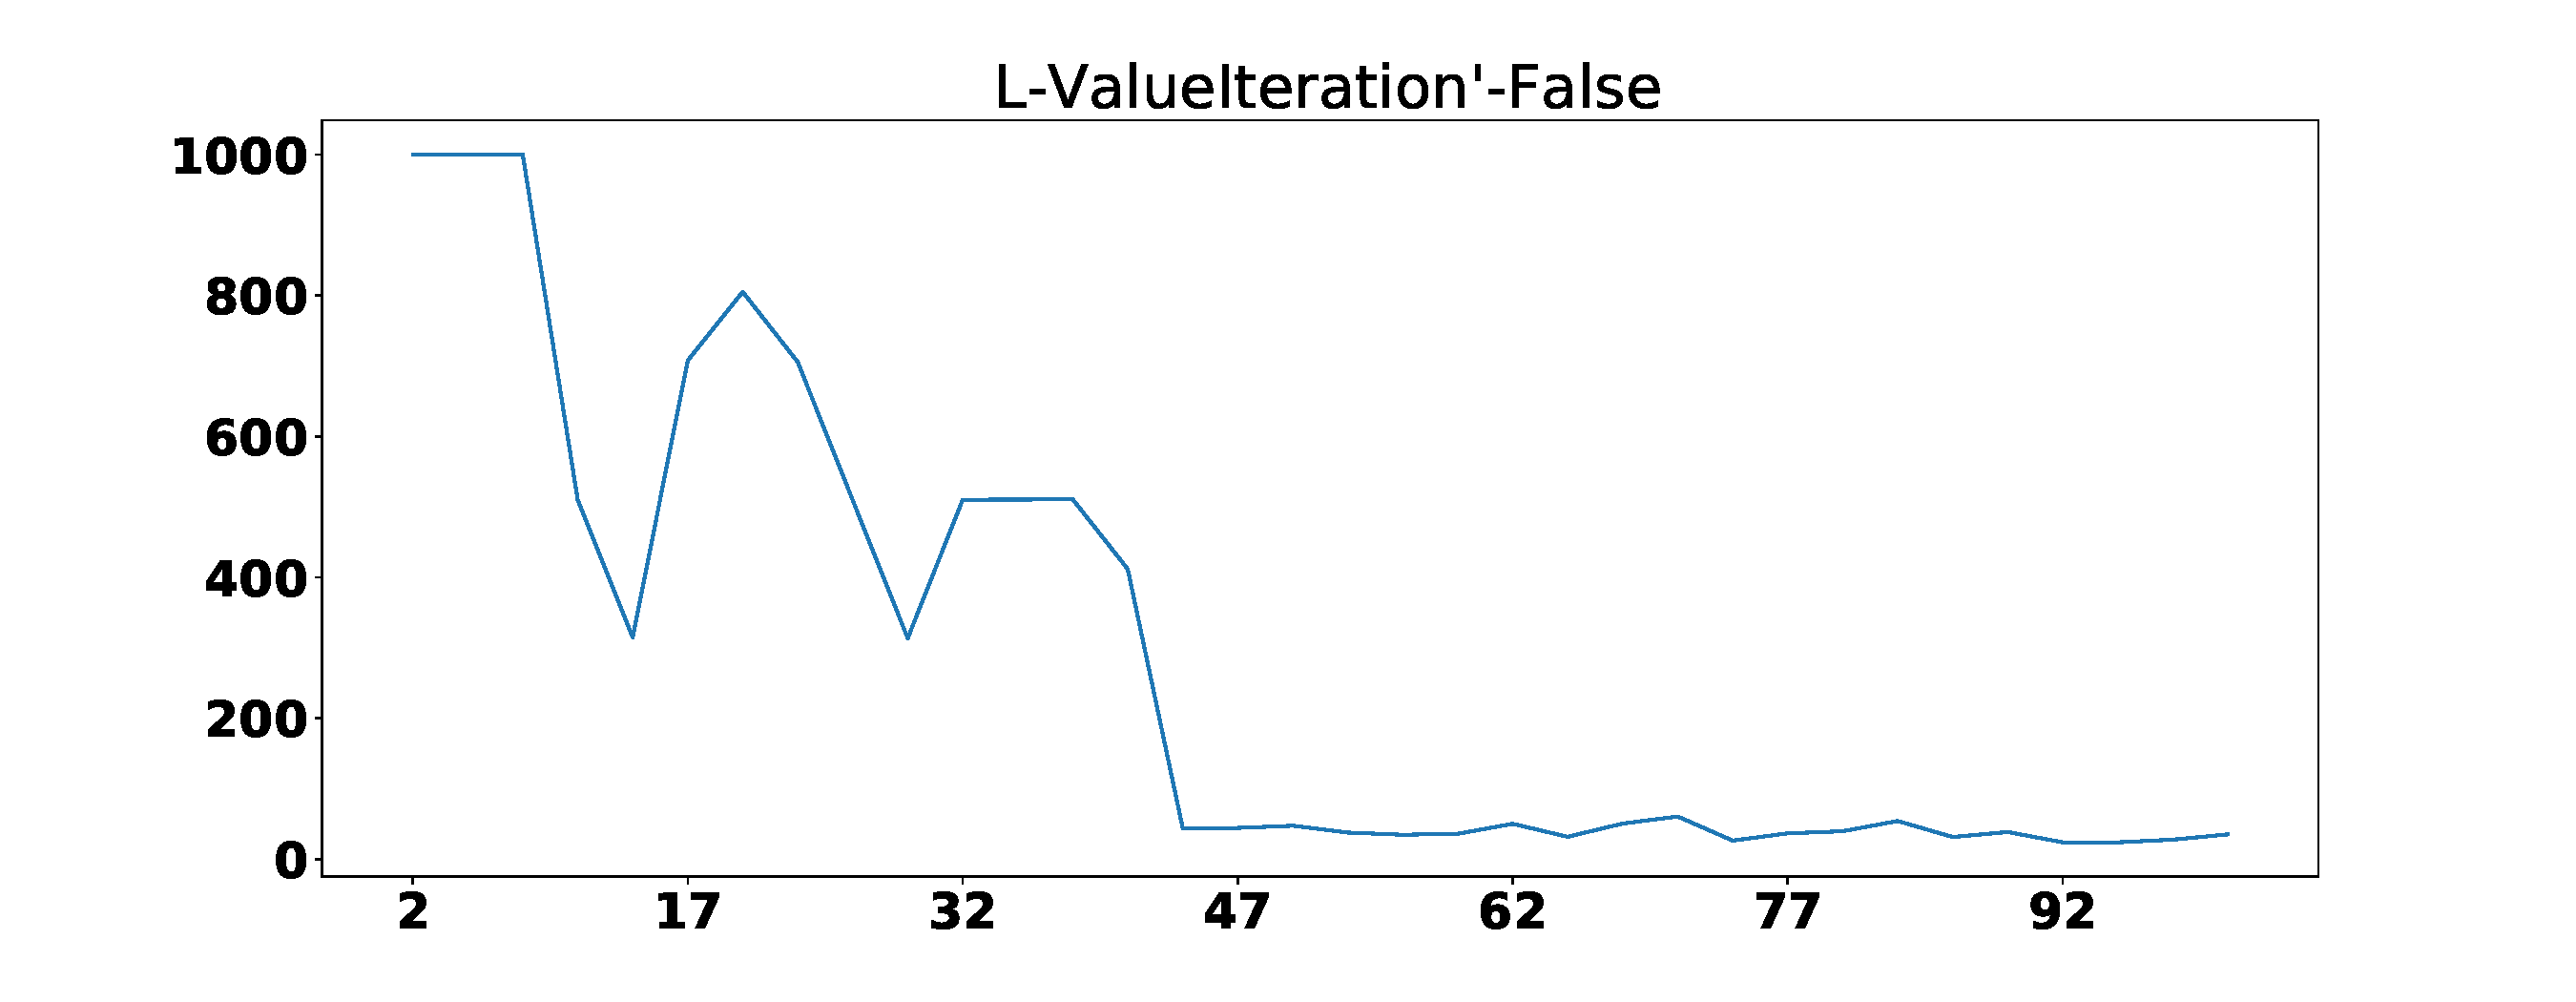
\includegraphics[width=\textwidth]{Ltrack_1_learning_rate.pdf}
    \end{subfigure}
    \begin{subfigure}[t]{0.3\textwidth}
    \centering
    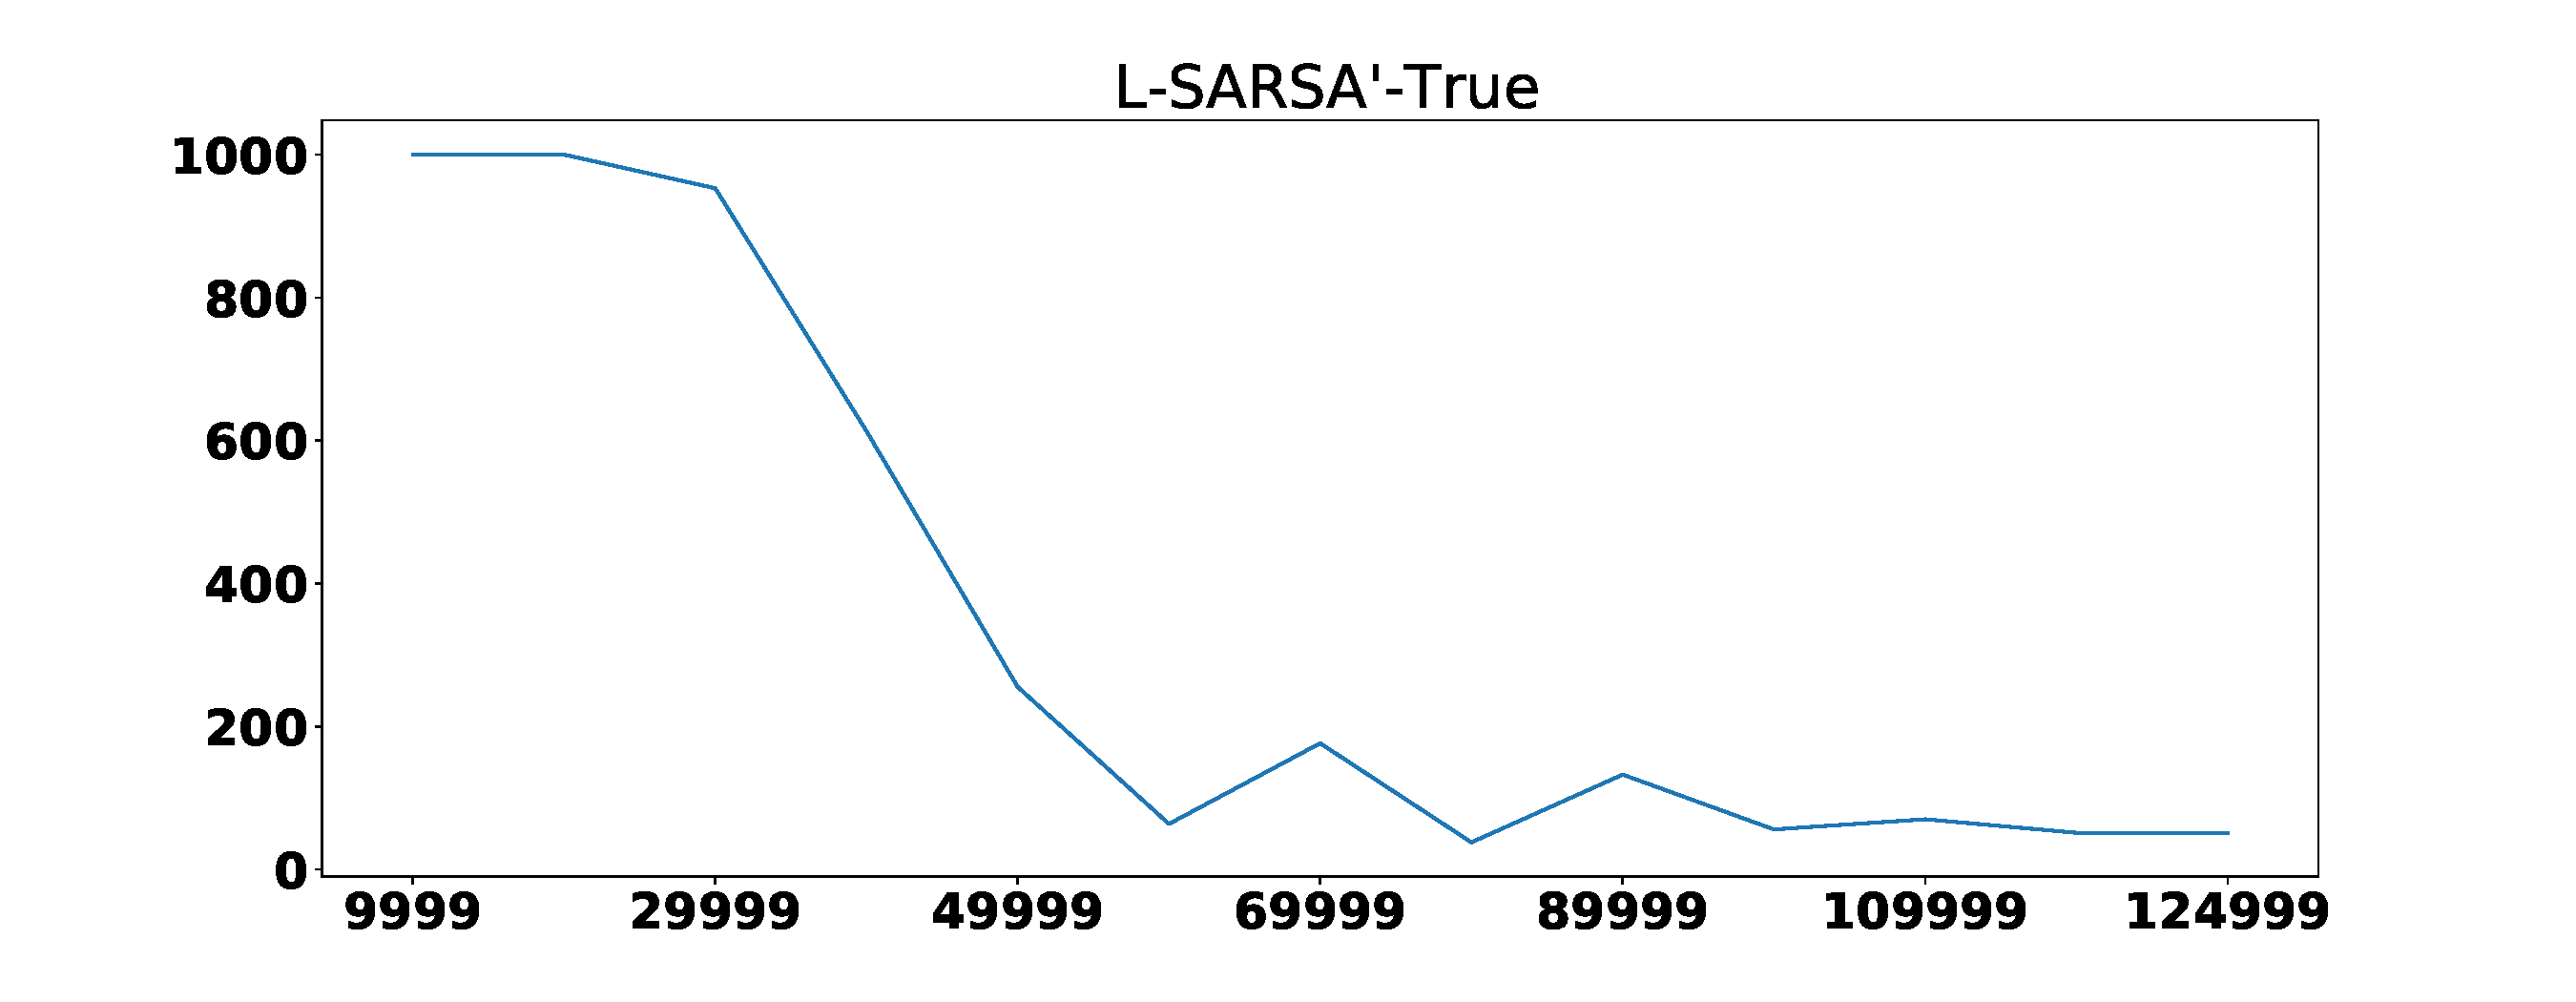
\includegraphics[width=\textwidth]{Ltrack_4_learning_rate.pdf}
    \end{subfigure}
    \caption{This figure shows the average number of steps needed to solve the track after a given number of
    training iterations for each of the 6 L-track algorithm and crash variant combinations. Note that the exploitation
    step is limited to 1000 steps at maximum. 10 exploitations were run for each starting point on the track.}
    \end{figure}

    \section{Algorithm Behavior}

\bibliographystyle{plainurl}
\bibliography{biblio}
\end{document}